\section{Experiments}
\label{sec:experiments}

\subsection{Setup}
\label{sec:setup}

\paragraph{Benchmarks.}
We evaluate on \osw~\cite{xie2025jedi} (Ubuntu desktop), \sspro~\cite{li2025screenspotpro} (high-resolution
professional applications on Windows, macOS and Linux) and \ssv~\cite{cheng2024seeclick} (mobile, desktop and
web), using a fixed random sample of 500 instructions per benchmark (\osw has 510 in total), identical for all
methods. No AX information is used.

\paragraph{Leakage filtering.}
OS-Atlas, MMBench-GUI and \ssv partly share their sources. We compute a 256-bit difference hash of every
evaluation and training screenshot and drop evaluation screens within 6 bits of any screenshot the ranker was
trained on: 3 of 248 \osw screens, none of the 500 \sspro screens and 130 of 384 \ssv screens. All numbers are
reported on the remaining screens (481 / 500 / 326 instructions). Filtering changes \cov{50} by at most 0.3 points.

\paragraph{Metrics.}
\emph{Coverage at $K$} (\cov{K}) is the fraction of instructions whose target is among the first $K$ options; an
option matches the target if its centre lies in the answer box or it overlaps the box with IoU $>0.3$ while being
at most $4\times$ its area (for point answers: it contains the point). Unlisted targets count as misses at every
$K$. \emph{Listed} is coverage of the unranked, uncapped list (the ceiling of any ranking). We also report the
number of icons among the first $K$, which is the number of captions the labelling stage must compute, and
latency on one NVIDIA A10G.

\subsection{Coverage and ranking}

\begin{table*}[t]
\centering
\small
\setlength{\tabcolsep}{4pt}
\begin{tabular}{l ccc ccc ccc}
\toprule
& \multicolumn{3}{c}{\osw} & \multicolumn{3}{c}{\sspro} & \multicolumn{3}{c}{\ssv} \\
\cmidrule(lr){2-4}\cmidrule(lr){5-7}\cmidrule(lr){8-10}
Ordering & \cov{10} & \cov{50} & caps@50 & \cov{10} & \cov{50} & caps@50 & \cov{10} & \cov{50} & caps@50 \\
\midrule
Detector order (unranked) & 6.0 & 38.9 & 10 & 2.4 & 21.0 & 16 & 35.0 & 92.6 & 14 \\
Random & 9.4 & 37.2 & 33 & 3.6 & 17.6 & 42 & 35.3 & 90.2 & 20 \\
Detector confidence & 15.6 & 39.5 & 32 & 7.2 & 31.0 & 40 & 51.8 & 93.9 & 17 \\
OCR text match & 29.1 & 55.9 & 10 & 27.6 & 56.6 & 19 & 69.6 & 95.4 & 15 \\
SigLIP zero-shot, tight crops & 37.6 & 57.4 & 26 & 43.2 & 59.8 & 38 & 84.4 & 96.3 & 19 \\
SigLIP zero-shot, context crops & 43.0 & 63.4 & 30 & 43.6 & 62.0 & 39 & 80.1 & 96.9 & 19 \\
\textbf{Ours} (fine-tuned, context, listwise) & \textbf{58.8} & \textbf{75.1} & 35 & \textbf{64.8} & \textbf{81.8} & 43 & \textbf{95.1} & \textbf{98.5} & 20 \\
\midrule
Listed (uncapped, any order) & \multicolumn{3}{c}{83.8 \quad (190 options)} & \multicolumn{3}{c}{96.0 \quad (442)} & \multicolumn{3}{c}{98.5 \quad (47)} \\
\bottomrule
\end{tabular}
\caption{\textbf{Coverage of the target at list length $K$} on leakage-filtered benchmarks, all orderings over the
same candidate lists. caps@50: median number of icons in the first 50 options, \ie captions needed.}
\label{tab:main}
\end{table*}

The candidate lists contain the target for 83.8\%, 96.0\% and 98.5\% of instructions (\cref{tab:main}). Without
the instruction, their order is close to random: the first 50 options by detector confidence contain the target
for only 39.5\% / 31.0\% of \osw / \sspro instructions. Lexical matching between the instruction and OCR text helps
for text targets but cannot see icons, and an off-the-shelf SigLIP scoring the candidates zero-shot reaches only
62--63\% \cov{50} on \osw and \sspro. Our ranker keeps the target in the first 10 options for 64.8\% of \sspro
instructions and in the first 50 for 81.8\%, which is 85\% of the listed targets. Its first 50 options contain a
median of 43 icons instead of 347. \Cref{fig:covk} shows coverage at every $K$.

\begin{figure*}[t]
\centering
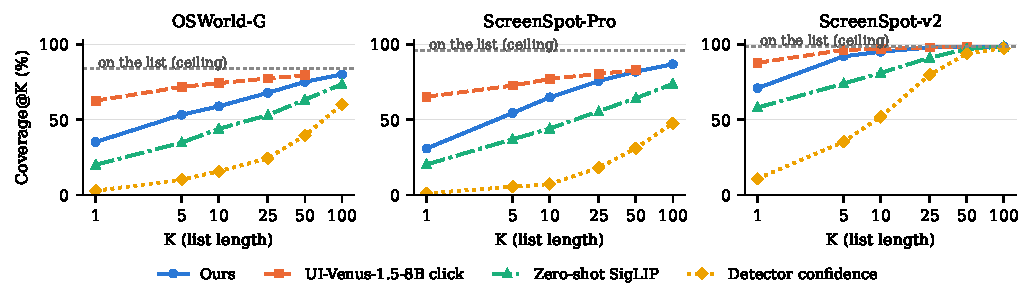
\includegraphics[width=\linewidth]{fig/cov_k.pdf}
\caption{\textbf{Coverage vs.\ list length} (leakage-filtered). Ours: 0.66 / 1.60 / 0.32~s per screen on an A10G; UI-Venus-1.5-8B's click turned into a ranking by distance: 1.57 / 2.98 / 2.16~s. The grounder is ahead at small $K$; at $K{=}50$ the gap is 4.3 / 1.0 / $-$0.3 points, at 1.9--6.8$\times$ lower cost, and fusing both is best (\cref{tab:grounders}). Dashed: the target is on the candidate list at all.}
\label{fig:covk}
\end{figure*}


\paragraph{What is still missed.}
On \sspro, almost all listed targets that our ranker places beyond 50 are small icons (target area below
$10^{-4}$ of the screen) on screens with more than 400 candidates. Recognising them requires knowing an
application's icon vocabulary, such as ``generate bitstream'' in Vivado or ``mark dimensions'' in SolidWorks, where
\cov{50} is only 42\%. On \osw, most remaining misses are relational instructions (``the second column of the
31st row'', ``the other text box'', ``the next slide''), which a ranker that scores each candidate independently
cannot resolve. A further 16\% of \osw targets are never listed: positions inside a slider or scrollbar, resize
grips and character spans. The supplement breaks coverage down by application group, element type and target size
(\cref{sec:supp-category}).

\subsection{Comparison with GUI grounding models}
\label{sec:grounders}

\begin{table*}[t]
\centering
\small
\setlength{\tabcolsep}{3.5pt}
\begin{tabular}{l c ccc ccc ccc}
\toprule
& & \multicolumn{3}{c}{\osw} & \multicolumn{3}{c}{\sspro} & \multicolumn{3}{c}{\ssv} \\
\cmidrule(lr){3-5}\cmidrule(lr){6-8}\cmidrule(lr){9-11}
Method & Params & click@1 & \cov{10} & \cov{50} & click@1 & \cov{10} & \cov{50} & click@1 & \cov{10} & \cov{50} \\
\midrule
TinyClick~\cite{pawlowski2024tinyclick} & 0.27B & 23.5 & 37.4 & 56.1 & 3.8 & 9.4 & 29.2 & 81.6 & 86.5 & 95.7 \\
ShowUI-2B~\cite{lin2025showui} & 2B & 21.0 & 48.6 & 66.3 & 7.6 & 40.8 & 59.4 & 76.7 & 91.1 & 96.9 \\
Qwen3-VL-2B & 2B & 32.4 & 45.3 & 60.9 & 30.2 & 45.6 & 61.8 & 81.6 & 88.3 & 96.6 \\
GUI-Actor-2B~\cite{wu2025guiactor} & 2B & 39.5 & 54.5 & 67.2 & 35.6 & 51.2 & 63.6 & 89.3 & 93.9 & 97.2 \\
UI-Venus-1.5-2B~\cite{gu2025uivenus} & 2B & 64.4 & 67.2 & 75.1 & 59.2 & 68.8 & 78.8 & 95.4 & 95.7 & 97.2 \\
UI-Venus-1.5-8B~\cite{gu2025uivenus} & 8B & 74.2 & 74.2 & 79.4 & 69.8 & 77.0 & 82.8 & 96.9 & 96.9 & 98.2 \\
\midrule
\textbf{Ours} & 0.2B & -- & 58.8 & 75.1 & -- & 64.8 & 81.8 & -- & 95.1 & 98.5 \\
Ours + UI-Venus-1.5-2B (fused) & & -- & 71.1 & 79.2 & -- & 72.8 & 88.4 & -- & 96.9 & 98.5 \\
Ours + UI-Venus-1.5-8B (fused) & & -- & \textbf{75.7} & \textbf{81.5} & -- & \textbf{77.8} & \textbf{89.0} & -- & \textbf{97.2} & \textbf{98.5} \\
\bottomrule
\end{tabular}
\caption{\textbf{Grounders as list builders.} click@1: the grounder's own click lands in the answer box.
\cov{K}: its click turned into a ranking of our candidates (candidates containing the click first, then by
distance). Fused: our score plus a Gaussian bonus around the click (fixed weight 5, width 0.5\% of the screen
diagonal for all benchmarks). All models run on the same instructions on one A10G; median latencies per
instruction in \cref{tab:speed}.}
\label{tab:grounders}
\end{table*}

Grounding models are trained to output one point, and every point induces a ranking: candidates under the point
first, then the rest by distance. \Cref{tab:grounders} evaluates six open grounders this way under our protocol.
Small, fast grounders (TinyClick, ShowUI) produce poor lists on dense screens because their single point says
little about the rest of the screen; their \cov{50} on \sspro is 29--59\%. Our ranker produces better lists than
every grounder up to 2B parameters except UI-Venus-1.5, at 2.3--9$\times$ lower latency than GUI-Actor-2B and
Qwen3-VL-2B (\cref{tab:speed}).

UI-Venus-1.5 is a much stronger grounder. Its click lands on the target for 74.2\% of \osw instructions, more than
our \cov{25}, but it fails on different instructions than our ranker. Adding a bonus around the grounder's click to
our scores gives the best lists at every $K$ on all three benchmarks: with UI-Venus-1.5-8B, \cov{10} rises to 75.7
/ 77.8 / 97.2\% and \cov{50} to 81.5 / 89.0 / 98.5\%. A list-based agent gets the grounder's pick first when it is
right. When it is wrong (26\% of \osw and 30\% of \sspro instructions), our ranking still has the target in its
top 10 for 25\% / 40\% of these misses and in its top 50 for 53\% / 64\%, which gives a selector a second chance.
Many of the remaining misses have no matching candidate at all (34\% of the UI-Venus-1.5-8B misses on \osw), and
no reordering can fix those.

\subsection{Downstream: a fixed selector}
\label{sec:selector}

Coverage is a proxy for whether the model that chooses from the list chooses correctly. To measure that directly,
we keep the selector fixed (Qwen2.5-VL-7B-Instruct without any fine-tuning) and vary only the list it receives. The selector
sees the screenshot (at most $1280\cdot28^2$ pixels), the instruction and the numbered options, each with its label
(OCR text, or the Florence-2 caption for icons) and its box, and answers with a number.

\begin{table*}[t]
\centering
\small
\setlength{\tabcolsep}{4pt}
\begin{tabular}{l rrrr rrrr rrrr}
\toprule
& \multicolumn{4}{c}{\osw} & \multicolumn{4}{c}{\sspro} & \multicolumn{4}{c}{\ssv} \\
\cmidrule(lr){2-5}\cmidrule(lr){6-9}\cmidrule(lr){10-13}
List given to the selector & cov. & acc. & ms & tok. & cov. & acc. & ms & tok. & cov. & acc. & ms & tok. \\
\midrule
Full list, unranked & 83.8 & 24.3 & 2118 & 6698 & 96.0 & 9.4 & 4043 & 13316 & 98.5 & 79.4 & 1004 & 2573 \\
Confidence, top 10 & 15.6 & 12.5 & 760 & 1562 & 7.2 & 4.2 & 763 & 1597 & 51.8 & 45.7 & 761 & 1609 \\
Confidence, top 50 & 39.5 & 20.8 & 1040 & 2607 & 31.0 & 12.8 & 1048 & 2685 & 93.9 & 76.7 & 995 & 2564 \\
Ours, top 5 & 53.2 & 37.8 & 729 & 1445 & 54.4 & 33.4 & 738 & 1457 & 92.0 & 79.4 & 742 & 1484 \\
Ours, top 10 & 58.8 & 37.6 & 760 & 1578 & 64.8 & \textbf{34.6} & 762 & 1595 & 95.1 & 80.1 & 761 & 1615 \\
Ours, top 25 & 67.8 & \textbf{38.5} & 841 & 1992 & 75.6 & 34.2 & 851 & 2008 & 97.9 & \textbf{81.0} & 843 & 2027 \\
Ours, top 50 & 75.1 & 37.4 & 1030 & 2690 & 81.8 & 31.6 & 1036 & 2702 & 98.5 & 79.4 & 1004 & 2564 \\
\bottomrule
\end{tabular}
\caption{\textbf{A fixed selector choosing from different lists} (Qwen2.5-VL-7B-Instruct, not fine-tuned;
leakage-filtered instructions as in \cref{tab:main}). cov.: a target is on the list; acc.: the selector picks a
target; ms: selector latency, median; tok.: prompt length, median. On \sspro, 4 of the 500 full lists do not fit
in GPU memory even with labels shortened to 25 characters; they count as errors.}
\label{tab:selector}
\end{table*}

The same selector does better with a better list (\cref{tab:selector}). On \osw, given every candidate, the
selector finds the target only 24.3\% of the time, although the target is on the list 83.8\% of the time: with 190
options it is right in only 29\% of the cases where it could be. Our top-10 list contains the target less often
(58.8\%), but the selector picks it far more reliably, for 37.6\% accuracy, with 4.2$\times$ fewer prompt tokens
and a 2.8$\times$ faster selector. The effect is larger on \sspro, where screens carry 442 candidates. There the
full list (13k tokens) gives 9.4\% and our top 10 gives 34.6\%, a 3.7$\times$ improvement with 8$\times$ fewer
tokens and a 5.3$\times$ faster selector. Shortening the list alone does not help: the top 10 by detector
confidence gives 12.5\% and 4.2\%. Accuracy is nearly flat from $K{=}5$ to $K{=}50$, because the gain in coverage is
offset by a harder choice (on \osw, accuracy when the target is listed falls from 71\% at $K{=}5$ to 50\% at
$K{=}50$). In practice $K$ can therefore be set by the latency and captioning budget. On \ssv, with 47 candidates
per screen, the full list is already short, and our top 10 matches its accuracy (80.1\% vs.\ 79.4\%) with
1.6$\times$ fewer tokens. Ranking helps most on dense screens.

A 7B selector choosing from our list remains below the best single-point grounders on these benchmarks
(UI-Venus-1.5-2B clicks correctly 64.4\% of the time on \osw). This experiment isolates the effect of the list. It
does not show that an untrained selector choosing from a list beats a trained grounder. Two ways to combine both
are selectors trained for option lists and the fused lists of \cref{sec:grounders}, which put a grounder's click
first and our ranked alternatives after it.

\subsection{Latency}
\label{sec:speed}

\begin{table}[t]
\centering
\small
\setlength{\tabcolsep}{4pt}
\begin{tabular}{l rrr}
\toprule
Stage (median ms) & OSW-G & SS-Pro & SS-v2 \\
\midrule
Candidates per screen & 190 & 442 & 47 \\
OCR (laptop)$^\dagger$ & 150 & 213 & 140 \\
Detection (2 detectors) & 190 & 254 & 179 \\
Merge & 14 & 35 & 4 \\
Context crops (GPU) & 15 & 43 & 8 \\
Image embeddings & 485 & 1121 & 120 \\
Text embedding + ranking & 11 & 12 & 11 \\
\textbf{Total (GPU)} & \textbf{656} & \textbf{1596} & \textbf{318} \\
\midrule
TinyClick & 132 & 151 & 140 \\
ShowUI-2B & 749 & 768 & 752 \\
UI-Venus-1.5-2B & 874 & 2614 & 1182 \\
GUI-Actor-2B & 1729 & 8694 & 2872 \\
Qwen3-VL-2B & 2433 & 3743 & 2414 \\
UI-Venus-1.5-8B & 1569 & 2976 & 2160 \\
\bottomrule
\end{tabular}
\caption{\textbf{Latency} per instruction on one A10G (OSW-G: \osw, SS-Pro: \sspro, SS-v2: \ssv; 100 screens per benchmark for ours, the 500 evaluation
instructions for the grounders, batch size 1). $^\dagger$OCR runs on the device that captured the screen,
concurrently with detection, and is not part of the GPU total.}
\label{tab:speed}
\end{table}

\Cref{tab:speed} breaks down our latency. Embedding the candidate crops takes most of the time and grows with the
number of candidates: 485~ms for the 190 candidates of a median \osw screen and 1.1~s for the 442 of a \sspro
screen. Two implementation choices matter. Cutting, resizing and normalising all crops on the GPU in one batched
\texttt{roi\_align} instead of with PIL removes about 0.5~s of CPU preprocessing per \sspro screen and changes
\cov{50} by at most 0.8 points (\cref{tab:ablations}). A vectorised merge gives identical lists in a tenth of the
time. End to end, our list costs 0.3--1.6~s per screen, 1.3--3.7$\times$ less than UI-Venus-1.5-2B and
1.9--6.8$\times$ less than UI-Venus-1.5-8B on the same GPU. The image embeddings can be reused, so a further
instruction on the same screen costs 11~ms. Labelling adds about 2~ms per captioned icon: on a median \sspro screen,
captioning the 43 icons in our top 50 takes about 90~ms, against about 0.7~s for all 347 icons (measured on 28
\sspro screens).

\subsection{Ablations}
\label{sec:ablations}

\begin{table}[t]
\centering
\small
\setlength{\tabcolsep}{2.5pt}
\begin{tabular}{l cc cc cc}
\toprule
& \multicolumn{2}{c}{OSW-G} & \multicolumn{2}{c}{SS-Pro} & \multicolumn{2}{c}{SS-v2} \\
\cmidrule(lr){2-3}\cmidrule(lr){4-5}\cmidrule(lr){6-7}
Variant & @10 & @50 & @10 & @50 & @10 & @50 \\
\midrule
Ours (384 px, 3 epochs) & 58.8 & 75.1 & 64.8 & 81.8 & 95.1 & 98.5 \\
\quad tight crops & 59.3 & 72.8 & 61.6 & 78.4 & 94.8 & 98.2 \\
\quad 224 px, 3 epochs & 61.1 & 74.4 & 58.2 & 77.4 & 94.8 & 98.2 \\
\quad 224 px, epoch 1 of 3 & 59.0 & 71.7 & 56.4 & 75.4 & 92.9 & 98.2 \\
\quad 224 px, 1 epoch & 60.9 & 73.2 & 60.0 & 76.6 & 94.2 & 98.2 \\
\qquad tight crops & 58.4 & 71.9 & 64.2 & 79.8 & 94.5 & 98.2 \\
\qquad sigmoid loss & 60.3 & 74.0 & 60.6 & 76.8 & 92.6 & 98.2 \\
\quad SigLIP2-so400m, 224$^\ast$ & 48.0 & 68.8 & 62.4 & 78.6 & 94.5 & 98.2 \\
\quad + Windows data$^\dagger$ & 62.2 & 74.8 & 65.6 & 82.2 & 95.1 & 98.5 \\
\quad GPU crops & 59.0 & 75.1 & 64.8 & 81.0 & 94.8 & 98.5 \\
\quad zero-shot, 384 & 43.9 & 63.2 & 44.0 & 64.2 & 81.0 & 96.9 \\
\bottomrule
\end{tabular}
\caption{\textbf{Ablations} (\cov{10} / \cov{50}, leakage-filtered). $^\ast$Lower 12 layers and embeddings frozen
to fit one 24\,GB GPU; saving the second epoch's checkpoint failed (disk full), so the evaluated weights are most likely the first epoch's. $^\dagger$7,651 training screens instead of 4,816, adding 2,979 OS-Atlas Windows screens; not used in the frozen model reported elsewhere.}
\label{tab:ablations}
\end{table}

\paragraph{Resolution.} Input resolution matters most on \sspro, where targets are smallest: going from 224 to
384 px adds 6.6 points of \cov{10} and 4.4 of \cov{50}, and changes \osw and \ssv by at most 2.3 points. Training
longer at 224 px helps on all three benchmarks (epoch 1 vs.\ epoch 3 of the same run).

\paragraph{Context vs.\ tight crops.} Without fine-tuning, the context window helps on \osw (+5.4 \cov{10},
\cref{tab:main}), where instructions often refer to an element's surroundings. After fine-tuning at 224 px the
results are mixed: context crops are better on \osw (+2.5 / +1.3) and worse on \sspro ($-$4.2 / $-$3.2). At 224 px
input, a window three times the element's size leaves a 16 px icon only a few pixels wide, so on \sspro the context
costs detail. At 384 px this cost disappears. Against tight crops trained identically, context crops gain 3.2 /
3.4 points on \sspro and 2.3 points of \cov{50} on \osw, and are within 0.5 points elsewhere. Context crops and the
higher resolution work together, which is why our model uses both.

\paragraph{Loss, data, encoder.} The per-screen listwise loss and a per-pair sigmoid loss perform alike (within
1.6 points everywhere). Both draw their negatives from the same screen, which seems to be the part that matters.
More data helps a little: adding 2,979 Windows screens raises \cov{10} by 3.4 points on \osw and 0.8 on \sspro,
with \cov{50} within 0.4 points. All other results use the model trained without them. A larger encoder does not
help within our budget: SigLIP2-so400m, with its lower half frozen to fit one 24\,GB GPU, is worse than the base
model on \osw and \sspro.

\paragraph{GPU crops.} Cutting and resizing crops on the GPU (\texttt{roi\_align}) instead of with PIL changes
\cov{50} by at most 0.8 points and removes the CPU preprocessing cost.
